
% TODO:
%   pow() function
%   .strip() string method
% memory diagrams -- diff between modifying in place and returning a copy (like
% .strip().)
% Left-side "variable names and atomic data". Right-side "aggregate data."

\chapter{Memory pictures}
\label{ch:memoryPictures}

Now that we've talked about the three important kinds of atomic variables,
let's consider the question of \textit{where they live}. It might sound like a
strange question. Aren't they ``in'' the Jupyter Notebook cell in which they
were typed?

Actually, no. And that brings me to the first mission-critical lesson of the
semester, which is a bane to all students who don't deeply grasp it. The lesson
is:

\begin{quote}
\textbf{The code itself is only a means to an end. The purpose of the code is
to read or write what's in memory.}
\end{quote}

\index{memory}
\index{environment}
\textbf{Memory} is the part of the computer in which variables and their values
are stored. To use the terminology of Chapter~\ref{ch:atomicData}, memory is
where the \textbf{environment} lives. It is \textit{invisible} to the
programmer, but it is also \textit{very much there.} The single most important
trick to learning how to write correct code is being able to summon to mind
what memory looks like at any point in time. The code you must write is a
natural consequence of that.

\section{A picture of memory}

\index{memory!picture}
It's easier with pictures at first, so we'll draw plenty of them. Our
\textbf{memory pictures} will have a very specific format, and this is
crucially important: don't get creative with how things are labeled or where
things are drawn. In order for your code to work \textit{you must have this
picture exactly right.} It's not art; it's science.

Our memory pictures will always be divided into exactly two ``realms,'' one on
the left and one on the right, labeled as follows:

\begin{center}
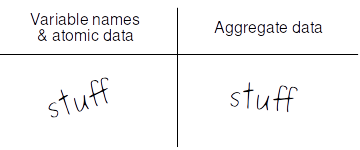
\includegraphics[width=.7\textwidth]{memoryPicture.png}
\label{fig:memoryPicture}
\end{center}

The left column's name should be recognizable, since that's exactly what we
covered last chapter. The right column won't have anything in it for a couple
chapters.

\subsection{Writing to memory}

When we create atomic variables in a Code cell, a la:

\begin{Verbatim}[fontsize=\small,samepage=true,frame=single,framesep=3mm]
pin_count = 844
username = 'Bekka Palmer'
\end{Verbatim}

each one gets put on the left-hand side of the diagram as a \textbf{named box}.
The name of the box is the variable's name, and the thing inside of the box is
its value.

\vspace{-.2in}
\begin{center}
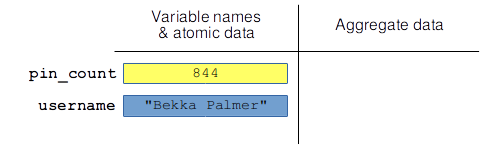
\includegraphics[width=.8\textwidth]{memoryPicture2.png}
\end{center}

It doesn't matter which boxes are higher or lower on the page, only that the
names stick with their boxes and don't get mixed up. As a bonus, I have colored
the boxes differently, indicating that \texttt{pin\_count} (an \texttt{int}) is
a different type than \texttt{username} (a \texttt{str}).\footnote{One other
tiny detail you might notice: even though our code had single quotes to delimit
Bekka Palmer's name, I put double quotes in the box in the memory picture. This
is to emphasize that no matter how you create a string in the code -- whether
with single quotes or double -- the underlying ``thing'' that gets written to
memory is the same. In fact, what's stored are actually the characters
\texttt{Bekka Palmer} \textit{without} the quotes. I like putting quotes in the
memory pictures, though, just to emphasize the string nature of the value.}

Creating more variables just adds more named boxes:

\begin{Verbatim}[fontsize=\small,samepage=true,frame=single,framesep=3mm]
...
avg_num_impressions = 1739.3
board_name = "Things to Make"
\end{Verbatim}

\vspace{-.2in}
\begin{center}
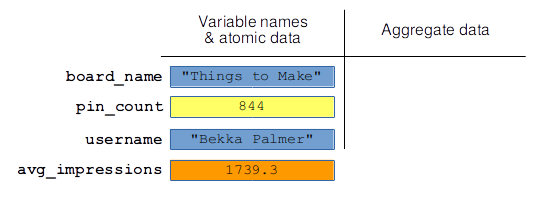
\includegraphics[width=.8\textwidth]{memoryPicture3.png}
\end{center}

I'm deliberately shuffling around the order of the boxes just to mess with you.
Python makes no guarantee of what ``order'' it will store variables in anyway,
and in reality it actually does become a big jumbled mess like this under the
hood. All Python guarantees is that it will consistently store a name, value,
and a type for each variable.

When we change the value of a variable (rather than creating a new one), the
value in the appropriate box gets updated:

\begin{Verbatim}[fontsize=\small,samepage=true,frame=single,framesep=3mm]
...
avg_num_impressions = 2000.97
pin_count = 845
another_board = 'Pink!'
\end{Verbatim}

\vspace{-.2in}
\begin{center}
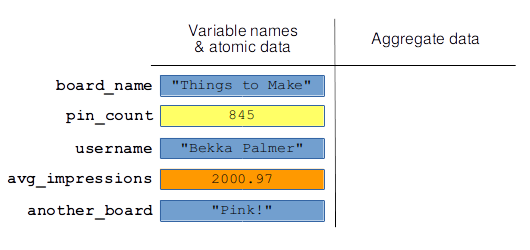
\includegraphics[width=.7\textwidth]{memoryPicture4.png}
\end{center}

Note carefully that \textit{the previous value in the box is completely
obliterated} and there is absolutely no way to ever get it back. There's no
way, in fact, to know that there even \textit{was} a previous value different
than the current one. Unless specifically orchestrated to do so, computer
programs only keep track of the present, not the past.

One other thing: unlike in some programming languages (so-called ``strongly
typed'' languages like Java or C++) even the \textit{type} of value that a
variable holds can change if you want it to. Even though the following example
doesn't make much sense, suppose we wrote this code next:

\begin{Verbatim}[fontsize=\small,samepage=true,frame=single,framesep=3mm]
...
pin_count = 999.635
username = 11
\end{Verbatim}

This causes not only the contents of the boxes to change, but even their
colors. The \texttt{username} variable was a \texttt{str} a moment ago, but now
it's an \texttt{int}.

\vspace{-.2in}
\begin{center}
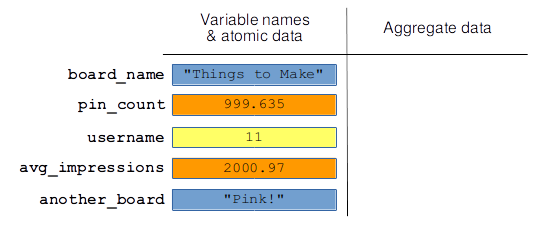
\includegraphics[width=.7\textwidth]{memoryPicture5.png}
\end{center}

\subsection{Reading from memory}

``Reading from memory'' just means referring to a variable in order to retrieve
its value. So far, we don't know how to do much with that other than print:

\begin{Verbatim}[fontsize=\small,samepage=true,frame=single,framesep=3mm]
print("The {} board has {} pins.".format(another_board, pin_count))
\end{Verbatim}

\begin{Verbatim}[fontsize=\small,samepage=true,frame=leftline,framesep=5mm,framerule=1mm]
The Pink! board has 999.635 pins.
\end{Verbatim}

The important point is that the memory picture is the (only) current, reliable
record of what memory looks like at any point in a program. Think of it as
reflecting a snapshot in time: immediately after some line of code executes --
and right before the following one does -- we can consult the picture to obtain
the value of each variable. This is exactly what Python does under the hood.

I stress this point because I've seen many students stare at complicated code
and try to ``think out'' what value each variable will have as it runs. That's
hard to do with anything more than a few lines. To keep track of
what-has-changed-to-what-and-when, you really need to maintain an up-to-date
list of each variable's value as the program executes...which is in fact
exactly what the memory picture is.

So if you're trying to figure out ``what will this program output if I print
the \texttt{odometer} variable immediately after line 12?'' don't stare at the
code and try to reconstruct its behavior from scratch. Instead, draw a memory
picture, update it accordingly as you walk through each line of code, and then
look at it for the answer.

\subsection{Tip}

By the way, investing in a small whiteboard and a couple of markers is a great
way to help you learn programming. They're perfect for drawing and updating
memory pictures as they evolve.

Hopefully this chapter was straightforward. These memory pictures will be
getting increasingly complex as we learn more kinds of things to store,
however, so stay sharp!
